\documentclass[
a4paper, % Stock and paper size.
12pt, % Type size.
% article,
% oneside, 
onecolumn, % Only one column of text on a page.
% openright, % Each chapter will start on a recto page.
% openleft, % Each chapter will start on a verso page.
openany, % A chapter may start on either a recto or verso page.
]{memoir}


%%% PACKAGES 
%%%------------------------------------------------------------------------------

\usepackage[utf8]{inputenc} % If utf8 encoding
% \usepackage[lantin1]{inputenc} % If not utf8 encoding, then this is probably the way to go
\usepackage[T1]{fontenc}    %
\usepackage[english,russian]{babel} % English please
\usepackage[final]{microtype} % Less badboxes

% \usepackage{kpfonts} %Font

\usepackage{amsmath,amssymb,mathtools} % Math

\usepackage[usenames,dvipsnames,svgnames,table,rgb]{xcolor}
\usepackage{tikz} % Figures. Following colors are predefined: red, green, blue, cyan, magenta, yellow, black, gray, darkgray, lightgray, brown, lime, olive, orange, pink, purple, teal, violet and white.

% Defining a new coordinate system for the page:
%
% --------------------------
% |(-1,1)    (0,1)    (1,1)|
% |                        |
% |(-1,0)    (0,0)    (1,0)|
% |                        |
% |(-1,-1)   (0,-1)  (1,-1)|
% --------------------------
\makeatletter
\def\parsecomma#1,#2\endparsecomma{\def\page@x{#1}\def\page@y{#2}}
\tikzdeclarecoordinatesystem{page}{
    \parsecomma#1\endparsecomma
    \pgfpointanchor{current page}{north east}
    % Save the upper right corner
    \pgf@xc=\pgf@x%
    \pgf@yc=\pgf@y%
    % save the lower left corner
    \pgfpointanchor{current page}{south west}
    \pgf@xb=\pgf@x%
    \pgf@yb=\pgf@y%
    % Transform to the correct placement
    \pgfmathparse{(\pgf@xc-\pgf@xb)/2.*\page@x+(\pgf@xc+\pgf@xb)/2.}
    \expandafter\pgf@x\expandafter=\pgfmathresult pt
    \pgfmathparse{(\pgf@yc-\pgf@yb)/2.*\page@y+(\pgf@yc+\pgf@yb)/2.}
    \expandafter\pgf@y\expandafter=\pgfmathresult pt
}
\makeatother

\usepackage{graphicx}  % Include figures
\usepackage{wrapfig}
\graphicspath{{img/}{../img/}}


%%% PAGE LAYOUT 
%%%------------------------------------------------------------------------------

\setlrmarginsandblock{0.15\paperwidth}{*}{1} % Left and right margin
\setulmarginsandblock{0.1\paperwidth}{*}{1}  % Upper and lower margin
\checkandfixthelayout

%%% SECTIONAL DIVISIONS
%%%------------------------------------------------------------------------------

\maxsecnumdepth{subsection} % Subsections (and higher) are numbered
\setsecnumdepth{subsection}

\makeatletter %
\makechapterstyle{standard}{
  \setlength{\beforechapskip}{0\baselineskip}
  \setlength{\midchapskip}{1\baselineskip}
  \setlength{\afterchapskip}{8\baselineskip}
  \renewcommand{\chapterheadstart}{\vspace*{\beforechapskip}}
  \renewcommand{\chapnamefont}{\centering\normalfont\Large}
  \renewcommand{\printchaptername}{\chapnamefont \@chapapp}
  \renewcommand{\chapternamenum}{\space}
  \renewcommand{\chapnumfont}{\normalfont\Large}
  \renewcommand{\printchapternum}{\chapnumfont \thechapter}
  \renewcommand{\afterchapternum}{\par\nobreak\vskip \midchapskip}
  \renewcommand{\printchapternonum}{\vspace*{\midchapskip}\vspace*{5mm}}
  \renewcommand{\chaptitlefont}{\centering\bfseries\LARGE}
  \renewcommand{\printchaptertitle}[1]{\chaptitlefont ##1}
  \renewcommand{\afterchaptertitle}{\par\nobreak\vskip \afterchapskip}
}
\makeatother

\chapterstyle{standard}

\setsecheadstyle{\normalfont\large\bfseries}
\setsubsecheadstyle{\normalfont\normalsize\bfseries}
\setparaheadstyle{\normalfont\normalsize\bfseries}
\setparaindent{0pt}\setafterparaskip{0pt}

%%% FLOATS AND CAPTIONS
%%%------------------------------------------------------------------------------

\makeatletter                  % You do not need to write [htpb] all the time
\renewcommand\fps@figure{htbp} %
\renewcommand\fps@table{htbp}  %
\makeatother                   %

\captiondelim{\space } % A space between caption name and text
\captionnamefont{\small\bfseries} % Font of the caption name
\captiontitlefont{\small\normalfont} % Font of the caption text

% \changecaptionwidth          % Change the width of the caption
% \captionwidth{1\textwidth} %

%%% ABSTRACT
%%%------------------------------------------------------------------------------

\renewcommand{\abstractnamefont}{\normalfont\small\bfseries} % Font of abstract title
\setlength{\absleftindent}{0.1\textwidth} % Width of abstract
\setlength{\absrightindent}{\absleftindent}

%%% HEADER AND FOOTER 
%%%------------------------------------------------------------------------------
\usepackage{nameref}
\makeatletter
\newcommand*{\currentname}{\@currentlabelname}
\makeatother

\makepagestyle{standard} % Make standard pagestyle

\makeatletter                 % Define standard pagestyle
\makeevenfoot{standard}{}{}{} %
\makeoddfoot{standard}{}{}{}  %
\makeevenhead{standard}{\bfseries\thepage\normalfont\qquad\small\leftmark}{}{}
\makeoddhead{standard}{}{}{\small\rightmark\qquad\bfseries\thepage}
% \makeheadrule{standard}{\textwidth}{\normalrulethickness}
\makeatother                  %

\makeatletter
\makepsmarks{standard}{
\createmark{chapter}{both}{shownumber}{\@chapapp\ }{ \quad }
\createmark{section}{right}{shownumber}{}{ \quad }
\createplainmark{toc}{both}{\contentsname}
\createplainmark{lof}{both}{\listfigurename}
\createplainmark{lot}{both}{\listtablename}
% \createplainmark{bib}{both}{\bibname}
\createplainmark{index}{both}{\indexname}
\createplainmark{glossary}{both}{\glossaryname}
}
\makeatother                               %

\makepagestyle{chap} % Make new chapter pagestyle

\makeatletter
\makeevenfoot{chap}{}{}{} % Define new chapter pagestyle
\makeoddfoot{chap}{}{}{}  %
\makeevenhead{chap}{\small\bfseries\thepage}{}{\hyperref[TOC]{Оглавление}}   %
\makeoddhead{chap}{\hyperref[TOC]{Оглавление}}{}{\small\bfseries\thepage}    %
\makeheadrule{chap}{\textwidth}{\normalrulethickness}
\makeatother

\nouppercaseheads
\pagestyle{standard}               % Choosing pagestyle and chapter pagestyle
\aliaspagestyle{chapter}{chap} %

%%% NEW COMMANDS
%%%------------------------------------------------------------------------------

\newcommand{\p}{\partial} %Partial
% Or what ever you want

%%% TABLE OF CONTENTS
%%%------------------------------------------------------------------------------

\maxtocdepth{subsection} % Only parts, chapters and sections in the table of contents
\settocdepth{subsection}

\AtEndDocument{\addtocontents{toc}{\par}} % Add a \par to the end of the TOC

%%% INTERNAL HYPERLINKS
%%%-------------------------------------------------------------------------------

\usepackage{hyperref}   % Internal hyperlinks
\hypersetup{
pdfborder={0 0 0},      % No borders around internal hyperlinks
pdfauthor={I am the Author} % author
}
% ----------- hyper ref -----------
\usepackage{hyperref}


\newcommand{\linkcolor}{blue}
\newcommand{\citecolor}{blue}
\newcommand{\filecolor}{magenta}
\newcommand{\urlcolor}{NavyBlue}
\hypersetup{				% Гиперссылки
	unicode=true,           % русские буквы в раздела PDF\\
	pdfstartview=FitH,
	colorlinks=true,  % false: ссылки в рамках; true: цветные ссылки
	linkcolor=\linkcolor,         % внутренние ссылки
	citecolor=\citecolor,        % на библиографию
	filecolor=\filecolor,      % на файлы
	urlcolor=\urlcolor,      % на URL
}
\usepackage{memhfixc}   %


%%% title page
\usepackage{pdfpages}
\ifpdf
  \usepackage{pdfcolmk}
\fi
%% check if using xelatex rather than pdflatex
\ifxetex
  \usepackage{fontspec}
\fi
\usepackage{graphicx}
%% for dingbats
\usepackage{pifont}
\newlength{\drop}% for my convenience

%% Generic publisher’s logo
\newcommand*{\plogo}{\fbox{$\mathcal{PL}$}}





\newcommand*{\titleJT}{\begingroup% Jan Tschichold: typographer
\drop = 0.08\textheight
\vspace*{\drop}
\hspace*{0.3\textwidth}
{\Large Александр Айвазян}\\[2\drop]
\hspace*{0.3\textwidth}{\Huge\itshape \textit{Еда: рецепты, советы и} }\par
{\raggedleft\Huge\itshape вегатерианство\par}
\vfill
\hspace*{0.3\textwidth}{
\includegraphics[width=0.1\linewidth]{img/isha_logo}}\\[0.5\baselineskip]
\hspace*{0.3\textwidth}{\Large }
\vspace*{\drop}
\endgroup}


%%% for beautiful icons
\usepackage{fontawesome}

\newenvironment{BiLines}
{\begin{samepage}\begin{center}
\begin{tikzpicture}
\draw[orange,thick] (0,0) -- (\textwidth,0);
\draw[orange,thick] (0,0.1) -- (\textwidth,0.1);
\end{tikzpicture}
\end{center}}
{\begin{center}
\begin{tikzpicture}
\draw[orange,thick] (0,0) -- (\textwidth,0);
\draw[orange,thick] (0,0.1) -- (\textwidth,0.1);
\end{tikzpicture}
\end{center}\end{samepage}}

\newenvironment{DidYouKnow}
{\begin{BiLines}
\textbf{\Large \faPencil\ Вы знали?}\\}
{\end{BiLines}}

\newenvironment{KeepInMind}
{\begin{BiLines}
\textbf{\Large \faLightbulbO\ Не забывайте}\\}
{\end{BiLines}}


%%% bibliography
\usepackage[backref=true]{biblatex}
\addbibresource{units/backmatter/mybib.bib}
\usepackage{csquotes}  % recomended to add

%%% indenting
\setlength{\parindent}{0em}
\setlength{\parskip}{0.5em}


%%%%%%%% Nice quote for recipes advice
% for adjustwidth environment
% \usepackage[strict]{changepage}

% for formal definitions
\usepackage{framed}

% environment derived from framed.sty: see leftbar environment definition
\definecolor{formalshade}{rgb}{0.95,0.95,1}

\newenvironment{formal}{%
  \def\FrameCommand{%
    \hspace{1pt}%
    {\color{darkgray}\vrule width 2pt}%
    {\color{formalshade}\vrule width 4pt}%
    \colorbox{formalshade}%
  }%
  \MakeFramed{\advance\hsize-\width\FrameRestore}%
  \noindent\hspace{-4.55pt}% disable indenting first paragraph
  \begin{adjustwidth}{}{7pt}%
  \vspace{2pt}\vspace{2pt}%
}
{%
  \vspace{2pt}\end{adjustwidth}\endMakeFramed%
}


%%%%
\usepackage{multicol}
\usepackage{paracol}
\usepackage{ifthen} 
\newenvironment{advice}
{%
\begin{formal}
\begin{itemize}%
}{%
\end{itemize}
\end{formal}%
}
%%%%% to center unnumbered subsections to create fancy recipe
\usepackage{titlesec}
% from the titlesec package
%\titleformat{ command }
%             [ shape ]
%             { format }{ label }{ sep }{ before-code }[ after-code ]
% \section*
\titleformat{name=\subsection,numberless}
{\filcenter\Large\bfseries}{}{0pt}{}
%{\vspace{-15pt} \hrulefill}{-13pt}    {\scshape\LARGE\bfseries}[\vspace{-25pt}]
\titlespacing*{name=\subsection,numberless}{0pt}{0pt}{-9pt}


\newcommand{\recipe}[8]
{%
\newpage
\subsection*{\emph{\huge #1}}
\addcontentsline{toc}{subsection}{#1}
%%% try to use just text, instead of sec, but sec is OK
% \par
% \noindent\makebox[\textwidth][c]{%
%     \begin{minipage}{0.6\textwidth}
%         \centering
%         \textbf{\emph{\huge #1}}
%     \end{minipage}
% 
% 
% }
% {\vspace{-30pt}

\faClockO\ \ifthenelse{\equal{#2}{}}{?}{#2} мин. \hfill \faSpoon\ \ifthenelse{\equal{#3}{}}{? литра (? порций)}{#3}
% }

\begin{tikzpicture}
\draw[gray,thick] (0,0) -- (\textwidth,0);
\draw[gray,thick] (0,0.1) -- (\textwidth,0.1);
\end{tikzpicture}

\begin{multicols}{2}
\textbf{\large Ингредиенты}
\begin{itemize}
#4
\end{itemize}
\vspace{100pt}

\columnbreak
\textbf{Специи}
\begin{itemize}
#5
\end{itemize}
\end{multicols}
\nointerlineskip

\textbf{\large Метод}

#6
#7

\ifthenelse{\equal{#8}{}}{}{%
\tikz[remember picture,overlay] \node[opacity=0.20,inner sep=0pt] at (page cs:0,-0.5){\includegraphics[height=0.5\paperwidth]{#8}};} 
}





\begin{document}
\pagestyle{empty}
\let\cleardoublepage\clearpage
%=======================================================================
\frontmatter
<красивая обложка>
\newpage
\setlength{\voffset}{1.5cm}
%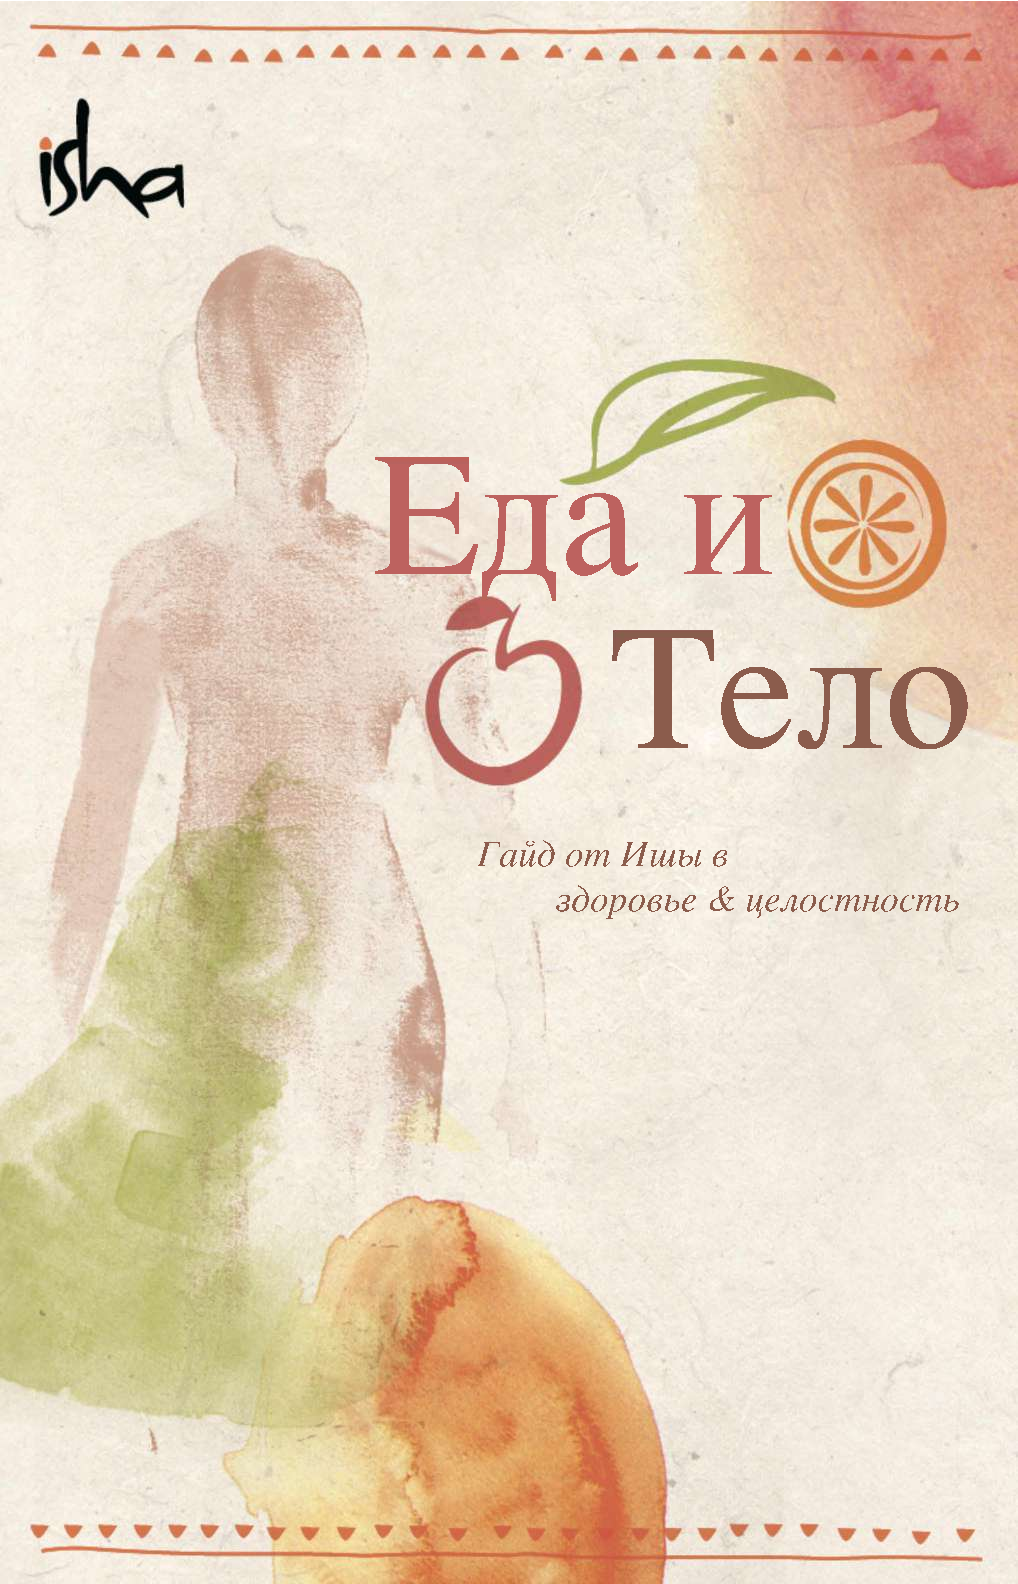
\includepdf[pages=1,width=\paperwidth]{img/FoodBody_cover_rus_compressed.pdf}
\setlength{\voffset}{0cm}

\titleJT
\cleardoublepage
\clearpage

\pagestyle{standard}
%%%colophon

\begin{abstract}	
%\raggedright
\noindent
\textbf{%
    Здоровое питание: советы \& простые рецепты\\
\textcopyright{2021 Sattva} \\
Первое издание: месяц 2021 года}\\[10pt]

\noindent
Все права защищены. Никакая часть этой книги не может быть воспроизведена в любой форме без письменного разрешения издателя, за исключением кратких цитат, содержащихся в критических статьях и обзорах.

\vspace{5pt}\noindent
Дизайн обложки, верстка, верстка книг и компиляция выполнены волонтерами организации Sattva. Все фотографии, использованные в этой книге, являются либо собственностью организации Sattva, либо находятся в общественном достоянии.

\vspace{10pt}\noindent
%\textbf{Опубликовано:} Isha Foundation 15, Govindasamy Naidu Layout, Singanallur, Coimbatore - 641 005 ИНДИЯ

\noindent
\textbf{Телефон:}

\noindent
\textbf{Электронная почта:} 

\noindent

\vspace{10pt}\noindent
\textbf{Отказ от ответственности:} Вся информация, представленная в этой книге, предназначена только для информационных и образовательных целей и не должна толковаться как медицинская консультация или инструкция. Никакие действия не должны приниматься исключительно на основании содержания этой книги. Пожалуйста, проконсультируйтесь со своим врачом или квалифицированным медицинским работником по любым вопросам, касающимся вашего здоровья и благополучия, или по любым мнениям, выраженным в этой книге.
\end{abstract}

\cleardoublepage


\tableofcontents\label{TOC}
\clearpage

\pagestyle{chap}
\section{Введение}
Намаскарам, дорогой участник!
\\

Мы надеемся, что все, кто смог сегодня присоединиться к тренингу ‘Йога Вира’ теперь понимает, как поделиться этим с другими людьми!
Как упоминалось во время обучения, вам открыт доступ к набору \href{https://sites.google.com/ishafoundation.org/yogaveera-russian}{‘Йога Вира’}.

Мы просим вас относиться к набору с максимальной святостью и сохранять конфиденциальность содержимого. Пожалуйста, не делитесь этим ни с кем другим.
 
Вы также можете \href{http://ishaeu.org/21day-sadhana-RU}{присоединиться} к сеансам 21-дневной садханы с понедельника 31 мая по понедельник 21 июня.

Это возможность для нас собраться вместе для садханы и углубить опыт использования инструментов, которыми затем мы сможем делиться с другими.
\\

Пранам,

Команда ‘Йога Вира’ Россия


%==========================================================================	
\mainmatter

\chapter{Советы \& лайфхаки}

\section{Почему все так просто}

В моей подборке нет таких блюд, как щи или картошка, потому что я считаю их абсолютно пустыми, также нету блюд, которые готовятся по несколько часов, в несколько этапов, во фритюре и т.д. Я призываю вас уходить от подобной кулинарной глупости.

Да, я могу испечь печенье для мамы, и только потому, что она просит и я её очень люблю. Но это отнимает уйму времени и грязной посуды. Если вы мужчина и решили приготовить какие-нибудь пирожки, селедку под шубой или фалафель, то скорее всего либо выдохнетесь, либо вообще разочаруетесь и лучше купите эту чертову селедку в ближайшем магазе и забудете про кулинарию надолго. Если же вы женщина, то муж вам после такого угощения пожизненно обязан. Цените своё время!!!

Мне всегда больно смотреть на людей, которые тратят часы на приготовление блюда, которое того не стоит, просто не стоит. Подумайте: блинчики, пирожки и булочки, сложные салаты, фритюр, бурфи, жареный сыр, даже плов, жюльен и халава — это всё бесполезная трата времени, вред для здоровья и издевательство над едой. Ведь в итоге, как бы вы не старались, это окажется внутри, а балласт выйдет известным путём. Не становитесь заложниками времени и жертвами блюдомании. Оцените трезво, что действительно нужно вашему телу, а что навязано извне.

Поэтому\ldots

Я подобрал для вас полезные, простые и функциональные блюда, из которых можно составить полноценное меню на неделю. Описание сокращено до минимума, чтобы рецепт можно было за 2 секунды окинуть взглядом и понять принцип процесса.

\section{Про самообразование}

А теперь напишу о том, как сделать всё ещё проще и в радость. Некоторые советы для начинающих, чтобы популярные вопросы отпали сразу:
\begin{itemize}
\item  Купите хорошую доску, набор удобных для вас ножей, посуды и других инструментов, чтобы приготовление еды приносило радость, и не превращалось в каторгу. Вам скорее всего понадобятся: небольшой казан, посуда нержавейка с толстым дном 2х-3х объёмов, лопатка, глубокое сито с ушками + миска под него, половник, большая ложка, большой широкий нож, малый нож, картофелечистка, тёрка, электрический чайник, стационарный и погружной блендер с мельничкой, кофемолка, духовка, плита и силиконовый противень.
\item  Установите обратноосмотический фильтр, забудьте про накипь в чайнике и наслаждайтесь чистой водой.
\item  Помните, что газовая плита всегда лучше конвекторной, а живой огонь лучше газа.
\item  Поинтересуйтесь в интернете о том, как чистить привычные вам продукты и вы узнаете много нового. Хороший пример: арбуз, ананас, авокадо или гранат. Возможно я даже сделаю подборку видео на тему.
\item  Научитесь эффективно и быстро резать. Это сэкономит вам тысячи часов вашей жизни.
\item  Режьте продукты так, чтобы: они сохраняли вкус, помещались в ложку и быстро готовились.
\item  Если падает нож, не спешите его ловить.
\item  Храните крупы и специи, свежевыжатые соки, супы и приготовленные блюда герметично в контейнерах.
\item  Узнайте вообще, как и где лучше хранить разные продукты.
\item  Узнайте время варки продуктов.
\item  Пробуйте и нюхайте каждый продукт перед закладкой. Помните о сроках годности.
\item  Мойте крупу перед варкой.
\item  В сладкие блюда добавляйте щепотку соли, а в солёные немного сахара.
\item  Помните, что мука — это клей, а сахар — яд.
\item  Всегда ищите лучшие пути для выполнения привычных операций.
\end{itemize}

\begin{quote}
    \emph{``Для многих кулинария — это творчество. Но в мире творчества есть тысячи гораздо более интересных занятий для души. Помните, что это всего лишь пища и её главная задача — питать наше тело.''}

\end{quote}


\section{Универсальный язык хорошего вкуса}

Итак, сегодня раскрываю секреты\ldots которые секретами не являются.
Как же сделать пресное блюдо привлекательным? 
Очень просто: наделить его всеми шестью вкусами — солёным, сладким, кислым, горьким, вяжущим и острым. На этом всё, спасибо за внимание, до свидания\ldots Шучу, читаем дальше!

Как известно, в ведической традиции считается, что основная трапеза должна содержать все 6 вкусов. Я с этим утверждением абсолютно солидарен, хоть и не приветствую соль. Когда эти вкусы гармонично взаимодействуют, человек получает весь спектр эмоций, потому что по сути, вкус~--- это эквивалент эмоции, и как только вы поймёте это, вам станет ясно, почему иногда хочется шоколадки, а иногда и хрена с чесноком. В другом случае, это потребность физиологического характера, например в период очищения или дефицита определённых веществ.

Так вот. Есть блюда, любимые многими, такие как плов, например. Я здесь не рассматриваю мясо, потому что с ним можно хоть гвозди есть, всё равно будет вкусно. Речь о вегетарианском варианте. Чтобы вы поняли, что делает безвкусный рис таким вкусным, надо просто проанализировать состав плова:
\begin{itemize}
\item Соль — солёный
\item Морковь, изюм, курага и чернослив — сладкий
\item Барбарис — кислый
\item Куркума, шафран — горький
\item Кумин — вяжущий
\item Лук и чеснок — острый
\item ну и Рис между делом, как сорбент всей композиции
\end{itemize}

Я думаю, вы теперь поняли, что рис без специй будет напоминать что-то вроде риса из студенческой столовки. Плов не самый лучший пример, но показательный. Я не считаю рис достойным продуктом для употребления, но на востоке в этом очень преуспели.

Теперь вы можете понять почему базу составляют всего несколько специй.

Другой пример — салат с рукколой и черри. Здесь всё дело в соусе по тому же принципу:
\begin{itemize}
\item оливковое масло, 2 стл
\item лимонный сок, 2 стл — кислый
\item гранатовый соус или шиповника, 1 стл — сладкий
\item чёрный перец, щепотка — острый
\item прованские травы, 1 чл — вяжущий
 
\item руккола — горький
\item сушёные помидоры — солёный
\end{itemize}


Заправка для Греческого салата:
\begin{itemize}
\item 3 чл оливкового масла
\item 3 чл лимонного сока
\item 1 зуб чеснока
\item 1/4 чл орегано
\item 1/4 чл соли
\item Сладость даёт болгарский перец
\end{itemize}

Ещё один вариант соуса:
\begin{itemize}
\item Растительное масло, 2 стл
\item Чеснок, 4 зуб.
\item Соевый соус, 4 стл
\item Лимонный сок, 2 чл
\item Мёд, 1 чл
\item Черный перец, 2 щеп.
\item Зелень, горсть.
\end{itemize}

Как вы видите, соусы содержат в себе почти все вкусы, а недостающие восполняют овощи и фрукты. Вообщем, принцип понятен.

Я заметил, что добавляя в блюдо чеснок, оно буквально преображается. Можно долго рассуждать о его раджастической природе, что это продукт в гуне невежества и прочее-прочее, но мы живём на земле, в конце концов. Особо просветлённые могут заменить его асафетидой. Чеснок, горький и острый одновременно, делает блюдо аппетитнее, это факт. В ресторанах вместе с лавашом часто подают пиалу с чесночным маслом. А на столе всегда есть соль, сахар и перец и лимон.

Специи~--- самый доступный способ сделать блюдо богаче. Только не сублимируйте эмоциональный вакуум — любимое дело гораздо важнее еды! Любите себя и дарите любовь.


\begin{figure}[ht]
    \centering
    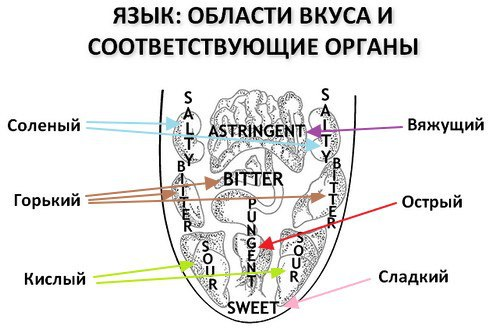
\includegraphics[width=0.6\textwidth]{img/SixTastes}
    \label{fig:1}
\end{figure} 

\section{Про специи}
Сегодня я хотел бы поговорить о специях и о том, как их выбирать и хранить. Об их свойствах я рассказывать не буду, потому что это долго, неинтересно и больше про лечебные свойства, что в наш динамичный мир не вписывается. Поскольку большинство людей — заложники вкуса, то лишь его и обозначу. Ниже перечислю основные специи, как говорится must-have, которые должны быть всегда под рукой.

БАЗА:

Кумин (зира) — вяжет: в основном, для бобовых
Кориандр (семена кинзы) — для овощей и нотки «бородинского»
Корица — делает всё слаще
Чили — жгучая острота
Чёрный перец — грубая острота
Ванильный сахар — делает выпечку сексуальнее
Соль — делает так, что хочется ещё
Сахар — без комментариев
Мёд — сладость без вреда
Лимон — добавляет кислинку
Чеснок — делает всё аппетитнее, остро-горький
Зелень (кинза, петрушка, укроп, руккола) — вкус, аромат и полезная горечь

НА РЕДКИЙ СЛУЧАЙ:

Куркума — для овощей
Гвоздика — для выпечки
Мускат — универсален
Имбирь — острый, универсален
Бадьян — пряный, для напитков
Хмели-сунели — для каш
Розовый перец — для супа
Прованские травы — для салатов
Орегано — для помидоров
Лавровый лист — для супа

ЦЕЛЫЕ ИЛИ МОЛОТЫЕ?

Целые предпочтительнее, т. к. дольше сохраняют аромат и вкус. Поэтому лучше иметь кофемолку и молоть самостоятельно. Однако есть специи, которые смолоть в обычной кофемолке не получится, поэтому надо брать готовый вариант. Обычно это Корица, Мускат, Куркума и другие твёрдые виды.

КАК ВЫБИРАТЬ И ГДЕ ПОКУПАТЬ:

Лучшие специи, на мой скромный взгляд, производит компания TRS. Приобрести их вы можете здесь: http://indianspices.ru или любом другом магазине специй. Если нет TRS, берите любые в герметичной упаковке. Всё, что продаётся на рынках в открытом виде — давно выветрилось и интереса не представляет.

КАК ХРАНИТЬ:

Самое простое — в аптечных контейнерах (видел также в Ашане по 15р/шт). Купите по одному большому для каждой отдельной специи. Это дёшево и практично. Всё остальное — маркетинг. В таком виде они хранятся указанный на упаковке срок.
Если блюдо содержит смесь специй, как плов или пряники, то композицию лучше готовить непосредственно перед закладкой.

ССЫЛКИ:

специи:
http://indianspices.ru 
http://ashaindia.ru/indiyskie-specii/
гималайская соль:
http://hpcsalt.ru

-------
Здесь я просто делюсь своим опытом. Большинство людей блуждают в потёмках невежества и до сих пор употребляют плоть животных. Надеюсь, что публикуемые рецепты вдохновят вас подняться на ступень выше, и взглянуть на свой рацион трезво.

Завтра я расскажу вам маленький секрет хорошего соуса, овладев которым, вы сможете сделать любое блюдо аппетитным… и объясню, почему в базу вошли указанные специи.


\newpage
\section*{Руководство к проведению онлайн сессий}
\label{sec:online}
\addcontentsline{toc}{section}{\nameref{sec:online}}

После прохождения онлайн-тренинга Йога Вира, у вас есть возможность проводить следующие модули онлайн:  % edit
\begin{itemize}
\item <<Йога для иммунитета>> (Саштанга и Симха крийя);
\item <<Йога для благополучия>> (Йога Намаскар и Нади Шуддхи);
\item <<Медитация для начинающих>> (Иша крийя);
\item Иша Упа йога (60 и 90 мин).

    Мы рекомендуем первые три сессии, так как большинство зрителей предпочитают менее 1 часа. Но если у них есть заинтересованная аудитория, они могут проводить и более длительные выступления.
\end{itemize}


Во время сессии вы можете поделиться с участниками \textbf{ссылкой на видео}, используя окно чата платформы для видеоконференций. Воспользуйтесь опцией
«Поделиться экраном» внутри платформы, которую вы используете для
проведения сессии, и воспроизведите видео.
Для каждой сессии нужно будет воспроизводить только одно видео.

Пожалуйста, выберите вариант сессии ниже и используйте подходящее видео по соответствующей ссылке. Вы можете использовать информацию о длительности видео (см. ниже), чтобы определить подходящий модуль для вашей сессии.
После выбора модуля, пожалуйста, \textbf{следуйте руководству} ниже.

\subsection*{Руководство}
\label{sec:list}
\addcontentsline{toc}{subsection}{\nameref{sec:list}}

\begin{enumerate}
    \item \textbf{Ознакомьтесь} с тем, какие виды сессий вы можете проводить самостоятельно.
    \item \textbf{Обратитесь за поддержкой} в Телеграмм-группу Йога Виры, если она вам
необходима.
\item \textbf{Предоставьте ссылки на часто задаваемые вопросы}, если они возникнут:
\begin{itemize}
    \item Иша крийя: \href{https://bit.ly/3fEbs13}{\tiny https://bit.ly/3fEbs13}
    \item Симха крийя: \href{https://isha.sadhguru.org/global/ru/simha-kriya/faq}{\tiny https://isha.sadhguru.org/global/ru/simha-kriya/faq}
    \item Саштанга: \href{https://drive.google.com/file/d/1LDbTnDl8uo3g3QCbMTGpZU-Kw2URPeEH/view?usp=sharing}{\tiny https://drive.google.com/file/d/1LDbTnDl8uo3g3QCbMTGpZU-Kw2URPeEH/view?usp=sharing}
\end{itemize}
\item \textbf{Отправьте напоминание участникам о следующем}:
    \begin{itemize}
    \item Приступайте к сессии на пустой желудок для практик Саштанга и Симха крийя.
    \item Приступайте к сессии на полупустой желудок для практик Йога Намаскар и Нади Шуддхи.
    \item Условие полупустого желудка рекомендовано, но не обязательно для сессии Иша крийи.
    А именно:
% \newpage
% \pagestyle{empty}
    \begin{itemize}
        \item[\faClockO] Должно пройти минимум 1,5 часа после полноценного приема пищи для 40/60/90 мин. сессий Иша Упа-йоги.
        \item[\faClockO] Должно пройти минимум 2,5 часа после полноценного приема пищи для сессий Симха крийи.
        \item[\faClockO] Должно пройти минимум 4 часа после полноценного приема пищи для сессий Саштанги.
    \end{itemize}
    \end{itemize}

\item \emph{Принимайте участие во всей сессии целиком.} Попросите всех участников участвовать во всей сессии целиком и оставаться до самого конца. Включая друзей и членов семьи \faSmileO.
\item \emph{Убедитесь, что вас ничто не отвлекает.} Важно, чтобы в течение следующих <упомянуть длительность (например, 40 минут)> не было никаких
помех. Это включает в себя использование телефона и походы в туалет. Мы
хотели бы начать сессию со знакомства с Садхгуру, а затем посмотреть
видео, где он объясняет практику и знакомит нас с ней. Пожалуйста,
следуйте инструкциям на протяжении всего видео.
\item \textbf{Используйте \hyperref[sec:plan]{этот сценарий}} для проведения вашей сессии.
% https://drive.google.com/file/d/1LDbTnDl8uo3g3QCbMTGpZU-Kw2URPeEH/view
\end{enumerate}

\paragraph{После сессии}
\begin{enumerate}
    \setcounter{enumi}{8}
\item \textbf{Поделитесь ссылкой на онлайн-программу «Внутренняя инженерия»}
  \href{https://www.innerengineering.com/ru/online}{https://www.innerengineering.com/ru/online} \faSmileO. Вы можете выбрать такой стиль общения, который будет уместен для ваших друзей и близких.
    \item \textbf{Благодарность.} И, наконец, не забудьте поблагодарить их за участие и предоставленную вам возможность предложить им несколько минут йоги.
    \item \textbf{Заполните \href{https://forms.gle/q1N7jG4vBEWBmng86}{отчет}} после сессии. 
\end{enumerate}

\paragraph{Чего \emph{не} делать}
\begin{itemize}
    \item[\faRemove] \textbf{\emph{Не} создавайте собственную сессию или последовательность сессии.} Если у вас есть какие-то идеи, которые вы хотели бы рассмотреть, пожалуйста, сообщите нам sadhanasupport.russian@ishafoundation.org. \textbf{Пожалуйста, не применяйте} собственную последовательность и не предлагайте никаких других практик, которые не упомянуты в этом Приложении.
    \item[\faRemove] \textbf{\emph{Не} отвечайте на вопросы самостоятельно.} Если вы не прошли официальную подготовку для ответов на вопросы, пожалуйста, запишите все заданные вопросы, отправьте их по адресу sadhanasupport.russian@ishafoundation.org для того, чтобы получить ответы, и вернитесь с ответом к тем, кто задал вопросы.
    \item[\faRemove] \textbf{\emph{Не} обучайте ничему самостоятельно:} ни путем демонстраций практик, ни путем объяснений. Если у вас есть какие-то идеи, которые вы хотели бы рассмотреть~--- пожалуйста, сообщите нам.
\end{itemize}

\subsection*{Структура}
\label{sec:struct}
\addcontentsline{toc}{subsection}{\nameref{sec:struct}}

Для сессий используйте видео, доступные по ссылкам в перечне ниже. Также все видео-инструкции можно найти в \href{https://youtube.com/playlist?list=PLnqgRgprlYQgJwgTSo8M29l0aJHQG2Efg}{этом плейлисте} на официальном YouTube канале Садхгуру.
\begin{itemize}
\item \href{https://drive.google.com/file/d/1OKuzlk67PiygUcywCozbgIGB38TLH6sv/view?usp=sharing}{Йога для иммунитета (видео 24 мин)}: 

    Саштанга + Симха крийя

\item \href{https://drive.google.com/file/d/1ONdlaZQIkNHkhtjV2z1Zkuut3AXz9Fys/view?usp=sharing}{Медитация для начинающих (видео 36 мин)}: 

    Иша крийя

\item \href{https://drive.google.com/file/d/1ONYEw1Z5vYU1K8JGLy2UkQTufU0hSr7u/view?usp=sharing}{Йога для благополучия (видео 37 мин)}: 

    Йога Намаскар + Нади Шуддхи


\item \href{https://drive.google.com/file/d/1O04lLBSqTakuITimFwo7eY6tpjlL3JV-/view?usp=sharing}{Иша Упа йога (видео 63 мин)}: 

    Движение рук по направлениям + Практики для шеи + Йога Намаскар + Нади Шуддхи
    

\item \href{https://youtu.be/Gseq7N49-JI}{Иша Упа йога (видео 86 мин)}: 

    Движение рук по направлениям + Практики для шеи + Йога Намаскар + Нади Шуддхи + Нада Йога + Шамбхави Мудра\footnote{Это не то же самое, что и Шамбхави Махамудра крийя.} + Практика Намаскар
\end{itemize}

% \begin{table}[ht!]
% \centering
% \begin{tabular}{|| p{0.48\linewidth} p{0.42\linewidth} | p{0.09\linewidth} ||}
%  \hline
%  \rowcolor{lightgray} \textbf{Сессия} & \textbf{Практики} & \textbf{Длина видео}  \\ [0.5ex]
% \hline\hline
% \href{https://drive.google.com/file/d/1OKuzlk67PiygUcywCozbgIGB38TLH6sv/view?usp=sharing}{Йога для иммунитета (45 мин)} & \href{https://youtu.be/RkWUAzPPuZ0}{Саштанга + Симха крийя} & 24 мин \\
% \hline
% \href{https://drive.google.com/file/d/1ONdlaZQIkNHkhtjV2z1Zkuut3AXz9Fys/view?usp=sharing}{Медитация для начинающих (60 мин)} &  \href{https://youtu.be/1VKDQraF82Y}{Иша крийя} & 36 мин \\
% \hline
% \href{https://drive.google.com/file/d/1ONYEw1Z5vYU1K8JGLy2UkQTufU0hSr7u/view?usp=sharing}{Йога для благополучия (40 мин)} & \href{https://youtu.be/aRxBafYDFo8}{Йога Намаскар} + \href{https://youtu.be/nfukQQqCM44}{Нади Шуддхи} & 37 мин \\
% \hline
% \href{https://drive.google.com/file/d/1O04lLBSqTakuITimFwo7eY6tpjlL3JV-/view?usp=sharing}{Иша Упа йога (65 мин)} &  \href{https://youtu.be/y-7UzbyJrR4}{Движение рук по направлениям} + \href{https://youtu.be/yuDuHILVl5Q}{Практики для шеи} + \href{https://youtu.be/aRxBafYDFo8}{Йога Намаскар} + \href{https://youtu.be/nfukQQqCM44}{Нади Шуддхи} & 63 мин \\
% \hline
% \href{https://youtu.be/Gseq7N49-JI}{Иша Упа йога (90 мин)} & \href{https://youtu.be/y-7UzbyJrR4}{Движение рук по направлениям} + \href{https://youtu.be/yuDuHILVl5Q}{Практики для шеи} + \href{https://youtu.be/aRxBafYDFo8}{Йога Намаскар} + \href{https://youtu.be/nfukQQqCM44}{Нади Шуддхи} + \href{https://youtu.be/vgA0W_FR5Ps}{Нада Йога} + \href{https://youtu.be/yvqJQDsw4bE}{Шамбхави Мудра\footnote{Это не то же самое, что и Шамбхави Махамудра крийя.}} + \href{https://youtu.be/Yv1J3QHObu8}{Практика Намаскар} 
% & 86 мин \\
% \hline
% \end{tabular}
% \caption{Структура сессий}
% \label{table:1}
% \end{table}


\subsection*{Профессиональный совет: простая платформа}
\label{sec:profAdv1}
\addcontentsline{toc}{subsection}{\nameref{sec:profAdv1}}

Вы можете использовать ту платформу, которая вам удобна. Если вы никогда раньше не пользовались платформами для видеоконференций, Google Meet — отличное бесплатное программное обеспечение, которое вы можете использовать. 

\href{https://drive.google.com/file/d/1aqEODSOCmS3BdFkcbs-sf_Aa1cjpd37d/view?usp=sharing}{Видео инструкции по использованию GoogleMeet.}

Если у вас есть платный аккаунт в Zoom, вы также можете использовать эту платформу для проведения сессий.

\href{https://drive.google.com/file/d/10llvQ_0aU7aWvye_Qvgj59LNMaya3aF8/view?usp=sharing}{Видео инструкции по использованию Zoom.}

\subsection*{Профессиональный совет: продвижение в социальных сетях}
\label{sec:profAdv2}
\addcontentsline{toc}{subsection}{\nameref{sec:profAdv2}}

Социальные сети предоставляют различные способы продвижения сессий в Интернете. Это важный шаг в организации сессии, потому что, если вы не обратитесь к аудитории, никто не узнает, что вы проводите сессию!
Если вы новичок в социальных сетях, не волнуйтесь \faSmileO. Пожалуйста, ознакомьтесь с рекомендациями ниже:
\begin{enumerate}
    \item \textbf{WhatsApp/Telegram.} Поделитесь деталями вашей сессии вместе со ссылкой на присоединение к группе через рассылку WhatsApp/Telegram.
    \item \textbf{VK/Facebook/Instagram.} Расскажите о своем мероприятии через пост И поделитесь деталями мероприятия через Сторис в Инстаграм в течение нескольких дней, предшествующих мероприятию.
\end{enumerate}


\faLightbulbO\ Если вы готовы, то самый эффективный способ обратиться к аудитории — через VK/Instagram Live.

\subsection*{Редактируемые приглашения: йога из дома}
\label{sec:invites}
\addcontentsline{toc}{subsection}{\nameref{sec:invites}}
Важно не редактировать первоначальные шаблоны. Пожалуйста, используйте \hyperref[sec:templates]{это руководство} по использованию шаблонов. 

Ниже приведены ссылки на шаблоны. Просто вставьте их в браузер и следуйте инструкции из \hyperref[sec:templates]{руководства}.
\begin{enumerate}\label{sec:templatesRefs}
    \item Шаблон для "Йоги для благополучия"\ \href{https://ishaeu.org/YVTemplateRU1}{\small https://ishaeu.org/YVTemplateRU1} 
    \item Шаблон для "Медитации для начинающих"\ \href{https://ishaeu.org/YVTemplateRU2}{\small https://ishaeu.org/YVTemplateRU2}
    \item Шаблон для "Йоги для иммунитета"\ \href{https://ishaeu.org/YVTemplateRU3}{\small https://ishaeu.org/YVTemplateRU3}  

\end{enumerate}



\chapter{Рецепты}
\textbf{СИСТЕМА МЕР}
\begin{itemize}
\item стакан — 250 мл
\item столовая ложка — 10 мл
\item чайная ложка — 5 мл
\end{itemize}
\begin{advice}
\item Топленое масло в рецептах можно заменить на кокосовое (для жарки) или любое другое растительное.
\end{advice}
\chapter*{Салаты}
\label{sec:salats}
\addcontentsline{toc}{section}{\nameref{sec:salats}}

Почему мало салатов?

Действительно, какая несправедливость!
Может быть, единственный салат, который вам пригодится в жизни~--- \hyperref[cleanSalat]{салат для очищения}.


Почему нет салатов из огурцов и помидоров и прочей дребедени? Потому что в отличие от приготовленных, свежие плоды употребляются отдельно, а в противном случае вызывают несварение, брожение и вздутие. Поэтому я исключил подобные кулинарные извращения во благо здоровья.

По этой же причине не найдёте здесь всеми любимой шарлотки и грибного супа, как изделий, вызывающих изжогу и запоры. По этой же причине я не пропагандирую хлеб, даже бездрожжевой.

По-хорошему, мне следовало бы исключить и кое-где фигурирующие молочные продукты, но постарайтесь почувствовать самостоятельно, что конкретно вам полезно, а что вызывает болезни. И прежде чем что-то исключать, найдите достойную альтернативу.
Об альтернативах можете \hyperref[sec:replace]{прочитать выше}.

Успехов!




%%% ================== recipe ================== %%%
\recipe{Салат для очищения}{5}{0.25}
{\label{cleanSalad}
\item морковь и китайская капуста поровну 250
\item масло растительное х/о 1-2 стл
\item зелень горсть
}{
\item кориандр 1/2 чл
\item чили 2 щепотки
\item мёд 1 чл
\item лимонный сок 10 мл
}{
Морковь на крупной тёрке, капусту и зелень порезать грубо, и заправить специями. Умножайте в несколько раз на большую кастрюлю.
}{
\begin{advice}
\item Почему морковь и китайская капуста? Потому что нейтрально, дёшево, эффективно и без побочных эффектов. 
\item Ничего другого, типа перца или помидоров, пожалуйста не добавляйте, т.к. всё равно не усвоится. 
\item Если вам скучно, поэкспериментируйте с другими корнеплодами и зеленью. Однако я уже третий год делаю один и тот же салат, и мне ещё не не наскучил.

\item Можно практически не жевать, потому что как вошёл, так и выйдет, но захватит с собой всё то, что в кишечнике быть не должно. Это грубая клетчатка – хорошая метла для тех, кто давно не чистился. Также можно есть в любое время суток, потому что ферменты здесь уже не участвуют.
\item Если у вас стул реже 3х-4х раз в день, — этот салат для вас. 
Гастроэнтерологи с противоположной точкой зрения могут идти мимо, не переубедите.


\item Через три недели ежедневного употребления салата оцените результаты. 

\end{advice}
}{cleanSalat}




%%% ================== recipe ================== %%%
\recipe{Морковь по-корейски}{5}{0.3}
{
\item сладкая морковь 250г
\item масло подсолнечное х/о 1 стл (по желанию)
\item сок лимона 1,5 стл
\item мёд 1 чл
\item кориандр молотый 1/2 чл,
\item кинза, горсть
}{
\item кунжут 1 стл,
\item чеснока зубчик 1 шт
\item перец черный 1 щеп,
\item перец чили 1 щеп,
\item соль 1/2 чл
}{
Морковь и чеснок потереть. Всё смешать и оставить в закрытой таре в холоде на 3-8 часов. Умножайте в несколько раз — съедается мгновенно!
}{}{carrot}



%%% ================== recipe ================== %%%
\recipe[Соус]{Салат с рукколой и черри}{5}{0.5}
{\label{arugula}
\item руккола 50
\item помидоры черри 400
\item сушёные помидоры (по желанию)
\item кедровые орехи, горсть
}{
\item оливковое масло, 2 стл (по желанию)
\item лимонный сок, 2 стл
\item гранатовый соус или шиповника, 1 стл
\item прованские травы, 1 чл
\item чёрный перец, щепотка
}{
Сделайте соус и добавьте к порезанным овощам.
}{
\begin{advice}
\item Да, можете туда кинуть какую-нибудь моцареллу или сулугуни.
\item Если нет кедровых~--- добавьте кешью.

\end{advice}}{salatTomato}{aaa}



\chapter{Рецепты}

\chapter*{Супы}
\label{sec:soup}
\addcontentsline{toc}{section}{\nameref{sec:soup}}

\newpage
\subsection*{\Large Чечевичный суп}
\label{sec:soupLent}
\addcontentsline{toc}{subsection}{\nameref{sec:soupLent}}
\faClockO\ 20 мин.

\textbf{\large Ингредиенты}
\begin{itemize}
\item 1/2 ст красной чечевицы
\item 3 ст кипятка
\item 2 горсти нарезанных помидоров
\end{itemize}

\textbf{Специи}
\begin{itemize}
\item 1/2 чл сахара (или 2 чл кокосового молока)
\item 1/2 чл зиры
\item 1 щепотка чили
\item 1 щепотка имбиря
\item 1 лавровый лист
\item 1 чл соли
\item 1 зуб чеснока
\item горсть кинзы
\end{itemize}

\textbf{\large Метод}

Чечевицу промыть, отварить со специями 12-15 минут. Помидоры и соль до кипения, выключить. Чеснок и зелень~--- в конце. % what? correct


\newpage
\section*{\Large Тыквенный суп}
\label{sec:soup2}
\addcontentsline{toc}{subsection}{\nameref{sec:soup2}}

\faClockO\ 5 мин.

\textbf{\large Ингридиенты}
\begin{itemize}
\item 2 ст. резаной тыквы
\item 2 ст. воды
\item 2 чл топлёнки
\item Горсть, тыквенные семечки 
\item 50 мл сливки (по желанию)
\item Зелень
\end{itemize}

\textbf{Специи}
\begin{itemize}
\item 1 чл тёртого имбиря
\item 1/4 чл зёрен горчицы
\item 1/4 чл куркумы
\item 2 щеп. черного перца
\item 2 щеп. муската
\item 1 чл соли
\end{itemize}


\textbf{\large Метод}

Тыкву в блендер. Обжарить в масле горчицу и имбирь 20 сек, добавить тыкву и специи, залить кипятком и поварить минуту. Выключить, разбить блендером, добавить сливки, семечки и рубленую зелень. 









\newpage
\section*{\Large Бобовый суп~--- самый сытный из супов}
\label{sec:soup2}
\addcontentsline{toc}{subsection}{\nameref{sec:soup2}}

\faClockO\ ? мин. \hfill \faSpoon\ 3 литра (7–10 порций)


\textbf{\large Ингридиенты}
\begin{itemize}
\item 4 банки консервированных красных бобов или 1,5 ст сухих
\item 5 ст кипятка
\item 1 стл растительного масла
\item 1 средняя луковица (по желанию)
\item 8 помидоров (ломтиками)
\item гарнир: петрушка, брынза
\end{itemize}

\textbf{Специи}
\begin{itemize}
\item 1 стл сушёного сладкого перца или помидоров
\item 1/4 чл сушёного острого красного перца
\item 1/2 чл розового молотого перца
\item 1 чл сухого орегано
\item 1 чл кумина (зиры)
\item 1 стл соли без горки
\item 3 зубчика чеснока (мелко)
\end{itemize}
\begin{formal}
\begin{itemize}
\item Специи лучше измолоть.
\end{itemize}
\end{formal}

\textbf{\large Метод}

Фасоль промыть, залить кипятком, довести до кипения, слить, промыть. Влить 5 ст. свежего кипятка, специи и на тихий огонь под крышку на 20 мин. В процессе пожарить лук, добавить. Подготовить помидоры, чеснок, соль, и добавить за 2 минуты. Подавать со свежей петрушкой и брынзой.

Если делаете из сухой фасоли, то замачивается на 6–8 часов, меняется вода, до кипения, вновь свежая вода и варится 1 час, либо экспресс методом по схеме 3+1: залить холодной водой и поварить 5 минут, оставить на 3 часа, слить и залить свежей водой, довести до кипения, вновь слить, залить свежей водой и варить 1 час.

 



\newpage
\section*{\Large }
\label{sec:soup2}
\addcontentsline{toc}{subsection}{\nameref{sec:soup2}}

\faClockO\ ? мин.

\textbf{\large Ингридиенты}
\begin{itemize}
\item 
\end{itemize}

\textbf{Специи}
\begin{itemize}
\item 
\end{itemize}


\textbf{\large Метод}


\newpage
\section*{Сценарий сессии}
\label{sec:plan}
\addcontentsline{toc}{section}{\nameref{sec:plan}}

\textbf{15 минут до начала сессии~---} откройте трансляцию (в зависимости от используемой платформы). 

\textbf{Ровно в назначенное время начала сессии~---} поприветствуйте участников, подждите пока все проверят свой звук и видео, переведите микрофоны (и видео) участников в бесшумный режим.

\textbf{Объявление, пока присоединяются другие участники}
\begin{quote}\emph{
Намаскарам/Доброе утро/Добрый день/Добрый вечер!
Добро пожаловать на сегодняшнюю сессию. Мы подождём ещё несколько
минут пока остальные участники присоединяются. Пока мы ждём, будет
лучше, если вы будете использовать наушники для участия в сессии и
оставите свои микрофоны в бесшумном режиме. (Если участникам нужна
помощь, вы можете сами перевести их микрофоны в бесшумный режим,
либо показать им как это сделать).
Доброе утро/день/вечер и добро пожаловать на сегодняшнюю
йога-сессию.
}\end{quote}

\textbf{На выбор~---} вы можете представиться, если участники с вами не знакомы.
\begin{quote}\emph{
Меня зовут \underline{\qquad} и я волонтёр Фонда «Иши» — международной
некоммерческой организации, основанной Садхгуру — йогином и
мистиком. Садхгуру предлагает мощные методы для само-преображения и
расширения своих возможностей через науку о йоге.
Я (назвать свою профессию: программист, инженер, домохозяйка, студент
итд) и на данный момент я работаю в \underline{\qquad}.
}\end{quote}

\begin{quote}\emph{
Сегодня я здесь для того, чтобы предложить вам простой набор практик,
спроектированных Садхгуру, которые позволят достичь физического и
психологического благополучия.
\\
Продолжительность этой сессии \underline{\qquad} минут.
\\
Чтобы извлечь максимальную пользу из своего участия в этой сессии, есть несколько вещей, которые вы можете сделать, чтобы создать благоприятную атмосферу. Пожалуйста, обратите внимание, что очень важно пройти эту сессию от начала до конца, так как предлагаемые практики должны изучаться систематически. Также мы просим вас не прерываться во время сессии на походы в туалет или использование телефона и не вставать.
\\
\textbf{(В зависимости от того, какая сессия проводится).} Определенные практики
требуют, чтобы их выполняли на полупустой желудок — должно пройти 1,5
часа после полноценного приема пищи (для Йога Намаскар) и 2,5 часа (для
Симха крийи). Если сейчас соблюдение этого условия для вас невозможно,
пожалуйста, не выполняйте эти практики и сделайте их, когда условие
полупустого желудка будет соблюдено.
\\
Сейчас Садхгуру даст необходимые рекомендации для практик. Сперва мы покажем короткое введение, а затем приступим к самим практикам. Сначала мы по смотрим демонстрацию, а затем перейдём к инструкциям для практик.
}\end{quote}

\textbf{Воспроизведите видео с практиками}
\begin{quote}\emph{
Мы надеемся, что вам понравилась сегодняшняя сессия. Эти практики
доступны на официальных каналах Садхгуру в YouTube. Просто следуйте
инструкциям из видео до тех пор, пока вам не станет комфортно выполнять
практики самостоятельно.
\\
Если у вас есть какие-либо вопросы по практикам, вы можете написать на
электронную почту: sadhanasupport.russian@ishafoundation.org (скиньте
адрес эл. почты в чат трансляции).
\\
Мы надеемся, что вам понравилась сегодняшняя сессия. Эти практики
доступны на официальных каналах Садхгуру в YouTube. Просто следуйте
инструкциям из видео до тех пор, пока вам не станет комфортно выполнять
практики самостоятельно.
Если у вас есть какие-либо вопросы по практикам, вы можете написать на
электронную почту: sadhanasupport.russian@ishafoundation.org \textbf{(скиньте адрес эл почты в чат трансляции)}.
\\
Если вы хотите исследовать науку о йоге во всей ее полноте и измерениях,
то следующий шаг, который мы рекомендуем предпринять, это наша
ведущая программа «Внутренняя инженерия». Онлайн-курс содержит 7
онлайн сессий, которые вы можете пройти вместе с Садхгуру в своём
темпе прямо у себя дома. Каждая сессия продолжительностью примерно
1,5 часа. После этого вы можете принять участие в Завершающей
программе, 3-дневном онлайн курсе, который включает передачу
Шамбхави Махамудра крийи — мощной очищающей 21-минутной
энергетической практики, которая объединяет дыхание вместе с
оздоравливающими и укрепляющими асанами.
\\
Если вы хотите узнать подробности программы, посетите официальный
сайт: \href{http://www.innerengineering.com}{\small http://www.innerengineering.com} \textbf{(поделитесь ссылкой в чате трансляции)}.
}\end{quote}

\textbf{По желанию}
\begin{quote}\emph{
Я бы хотел(а) поделиться с вами своим опытом от прохождения программы «Внутренняя инженерия».
\textbf{(Поделитесь своими впечатлениями и опытом от своей программы
«Внутренняя инженерия» согласно инструкциям, которые были даны во
время программы подготовки)}.
}\end{quote}

\textbf{По желанию}
\begin{quote}\emph{
Если вы хотите узнать больше о программе, пожалуйста, перейдите на сайт \href{http://www.innerengineering.com}{\small http://www.innerengineering.com} \textbf{(скиньте ссылку в чат трансляции)}. 
}\end{quote}

\begin{quote}\emph{
Спасибо за то, что приняли участие в сегодняшней сессии! Было очень приятно всех вас видеть. Если вы хотите узнать больше о подобных сессиях, вы можете найти их по ссылке, опубликованной в чате трансляции: \href{https://ishaeu.org/Yoga-veera-sessions-RU}{\small https://ishaeu.org/Yoga-veera-sessions-RU} \textbf{(скиньте ссылку в чат трансляции)}. 
}\end{quote}

\chapter*{Соусы}
\label{sec:sauces}
\addcontentsline{toc}{section}{\nameref{sec:sauces}}


%%% ================== recipe ================== %%%
\recipe{Айолли}{5}{0.35 кг}
{\label{aiolli}
\item Семечки подсолнуха сырые 300 мл
\item Кинза – 2 горсти
\item Соевый соус – 4 стл
\item Сок лимона – 4 стл
}{
\item Чеснок – 2 зуб
}{
Семечки измельчить в кофемолке, остальное в блендере, затем смешать. С хлебцами отлично!
}{
\begin{advice}
\item Берите соус Sensoy естественного брожения в стеклянной бутылке.
\item Паштет из семечек, нравится всем!
\end{advice}}{}



%%% ================== recipe ================== %%%
\recipe{Тахини}{5}{0.3 кг}
{\label{takini}
\item 1 стакан белого кунжута 
\item 1 стл кунжутного масла
\item 3 стл лимона
\item 2 стл петрушки
}{
\item 2 зуб чеснока
\item щепотка чили
\item 1/2 чл соли
\item 1/2 чл кумина (по желанию)
}{
Кунжут в кофемолке, остальное — в мельничке. Смешать. 
}{
\begin{advice}
\item Получается плотно, по вкусу прямо как сыр — можно на хлебцы намазывать.
\end{advice}}{}



%%% ================== recipe ================== %%%
\recipe{Ткемали из желтой сливы}{5}{250 г}
{
\item Слива жёлтая 300 г
}{
\item Семя кориандра, 1 чл
\item Семя укропа, 1 чл
\item Чеснок 1 небольшой зуб
\item чили, 1/4 чл
\item Соль, 1 чл
}{
Всё в блендер.  
}{
\begin{advice}
\item Очень вкусный соус! 
\end{advice}}{}



%%% ================== recipe ================== %%%
\recipe{Хренодёрка (хреновина)}{}{1 кг}
{
\item 1 кг вкусных помидоров
\item 40 г хрена
\item 3 стл лимонного сока
\item 2 чл мёда
}{
\item 50 г чеснока
\item 2 чл соли
\item 1/2 чл чили 
}{
Всё перетереть в мясорубке с крупной решёткой, закатать в стерильные банки.
}{}{khren}



%%% ================== recipe ================== %%%
\recipe{}{}{}
{
\item 
}{
\item 
}{
}{}{}




\chapter*{Десерты}
\label{sec:sweet}
\addcontentsline{toc}{section}{\nameref{sec:sweet}}



%%% ================== recipe ================== %%%
\recipe{Овсяный пирог}{35}{1}
{
\item 1 ст сахара
\item 1 ст кефира или сметаны
\item 90 г сливочного масла
\item 1.5 ст ц/з муки
\item 1.25 ст овсяных экспресс хлопьев % ???
\item горсть изюма
}{
\item 1 чл соды
\item 0.75 чл соли
\item 0.5 чл корицы
\item 1 чл ванильного сахара
}{
Смешать в указанном порядке. Вылить на противень, запечь $180^{\circ}$ 20 мин.
}{
\begin{advice}
\item Случай, когда гости приходят неожиданно.
\end{advice}}{}



%%% ================== recipe ================== %%%
\recipe{Полезное печенье}{5}{0.15}
{\label{cookies}
\item 100 г кунжута 
\item 50 г мёда
}{
\item 0.5 чл ванильного сахара
}{
Кунжут измельчить в кофемолке и все смешать.
}{
\begin{advice}
    \item  Жирненько, сладенько, пахнет выпечкой. По вкусу, как песочное тесто.
\item Если у вас аллергия на кунжут~--- покупайте чёрный нешлифованный~— он не отбелен известью. Если и на чёрный реакция, я вас поздравляю,~— вам надо очищаться, или же оставаться в комфортном болоте\ldots

\end{advice}}{}



%%% ================== recipe ================== %%%
\recipe[]{Живая халва за 5 минут}{5}{---}
{


\item подсолнух + мёд

    (можно с маком)
\item кунжут + мёд 

    (можно добавить ваниль)
\item абрикосовое ядро + мёд 

    (типичный марципан)

}{%
\item[]
}{
Принцип: семена + мёд в пропорции 2:1. Семена измельчаются в кофемолке. Варианты в ингредиентах.
Смешать в контейнере и там же хранить.
}{}{halva}



%%% ================== recipe ================== %%%
\recipe[]{Рафаэлло}{20}{0.2}
{
\item 100 г фиников

\item 50 г черногоизюма
\item 2 стл (20 г) кокосовой стружки 
\item Кокосовая стружка для обсыпки
}{
\item[]
    }{
Измельчить в мясорубке, смешать, накатать, обвалять в кокосовой стружке.  
}{
\begin{advice}
\item Можно ничего не катать и есть ложкой.
    \item Хранится в холоде.
        \item Брал финики Каспиан, изюм Изабелла. Стружку пробовать!

\end{advice}
}{raf}





%%% ================== recipe ================== %%%
\recipe{Апельсиновый шар {\normalsize (привет «Джаганнат»)}}{20}{0.15}
{
\item 100 г фиников
\item 40 мл зел. молотой гречки 
\item 2 чл какао
}{
\item 1 щеп свежей цедры апельсина
\item спичечная головка молотого кардамона
\item 1 щеп корицы
}{
Гречку в кофемолке, финики через мясорубку, всё смешать, накатать, обвалять в той же гречке или какао.
 
}{
\begin{advice}
\item Умножайте в несколько раз.
\item Пропорции не менять!
\end{advice}}{orangeBalls}




%%% ================== recipe ================== %%%
\recipe{Лимонные шары}{20}{0.13}
{
\item 100 г кураги
\item 20 г кокосовой стружки
\item 2 чл лимонного сока
\item Сверху сушёная лимонная цедра молотая
}{
\item 2 чл свежей мяты / 1 капля масла мяты
}{
Курагу через мясорубку, всё смешать, накатать, обвалять в цедре или стружке. 
}{
\begin{advice}
\item Умножайте в несколько раз.
\item Соблюдайте пропорции.
\end{advice}}{lemonBalls}







%%% ================== recipe ================== %%%
\recipe{Шоколад}{20}{0.1}
{
\item 10 г какао масло х/о
\item 100 г фиников
\item 5 г какао 
\item Молотая гречка для обсыпки
}{
\item  0.3 чл ванильной эссенции (концентрат)
}{
Гречку в кофемолке, финики через мясорубку, всё смешать, накатать, обвалять в гречке или какао. 
}{
\begin{advice}
\item Умножайте в несколько раз.
\item Соблюдайте пропорции.
\end{advice}}{choco}







% %%% ================== recipe ================== %%%
% \recipe{}{}{}
% {
% \item 
% }{
% \item 
% }{
% }{}{}
% 
% 
% 










\foodTitle{Напитки}{}



%%% ================== recipe ================== %%%
\recipe{Чай масала}{15}{1.3}
{
\item 3 ст кипятка
\item 2 ст нежирного молока
\item Свежий имбирь $1\times 3$ см (1 стл с горкой, 10г)
\item 3 стл (40г) сахарного песка
\item 3 стл с горкой (16г) черного чая <<Пуэр>>
\item Марлевые салфетки или мелкое сито
}{
\item 0.25 мускатного ореха
\item 6-8 (0.25 чл молотой) веточек гвоздики 
\item Корица молотая 1 чл (2г)
\item 20 семян (2 чл молотого) зеленого кардамона  (раздавить в ступе)  
\item 1 чёрный кардамон 
}{
В кастрюле залить кипятком специи, сахар и имбирь, варить 5 минут, всыпать чай и поварить ещё 5 минут. Влить молоко и довести до кипения. Процедить напиток через сито или марлю. Подавать горячим.
}{
\begin{advice}
\item Рецепт проверен временем и выверен по пропорциям. Для романтического вечера — самое то!
\item С осторожностью обходитесь с имбирём. Он усиливает не только острый запах кардамона, но и даёт острый вкус. Пробуйте напиток в процессе! Молоко почти не смягчает остроту. 
    \item Сушеный имбирь использовать не рекомендую.
    \item Для веганского варианта то же самое, только варить всё 10 минут без чая и молока (заменить просто водой), процедить и мёд в конце.
            \item Пуэр можно найти в любом чайном магазине или магазине специй. Сейчас проблем с этим нет. Берите, чтоб нравился аромат — обычно пахнет хорошим чернозёмом.
                \item Почему я отказался от чая? Потому что считаю его сильным закислителем и, по сути, таким же наркотиком, как и кофе.
\end{advice}
\newpage
~
}{tea}





%%% ================== recipe ================== %%%
\recipe{Яблочный напиток}{10}{0.75}
{
\item 1 яблоко
\item 500 кипятка
\item 1 стл сиропа шиповника («Холосас» из аптеки / 0.5 ст крепкого отвара шиповника + 1 чл сахара)

}{
\item 2 палочки корицы или 2 щепотки
\item 3 веточки гвоздики
\item 1 звездочка бадьяна
\item 1 щепотка черного перца
\item 1/2 чл ванильного экстракта или ванили
}{%
}{}{apple}




%%% ================== recipe ================== %%%
\recipe{Напиток из пажитника}{20}{1}
{
\item 1 л кипятка
\item мёд по вкусу
}{
\item 2 стл смян пажитника
}{
Семена варить 15 минут, процедить отвар и добавить мёд.
}{
\begin{advice}
\item Если выпить всю кастрюлю, 3 дня будете пахнуть пажитником \faSmileO. Благо аромат приятный \faSmileO.
\item Можно вообще на варить, а залить кипятком из расчёта 1 чл семян на стакан кипятка. Через 5 минут готов. Можно заваривать 2–3 раза. 
\end{advice}}{fenugreek}



%%% ================== recipe ================== %%%
\recipe[]{Напиток из шиповника}{100(10 работы)}{2}
{
\item 2 ст шиповника
\item 2 л воды
}{
\item[] 
}{
Шиповник варить в скороварке 1,5 ч.
}{
\begin{advice}
    \item Самый полезный напиток.
    \item Шиповник — классическое желчегонное наравне с брусникой.
\item Получается концентрированный отвар, который можно разбавлять и упиваться вместе с мёдом в течение дня и после 5 вечера, когда рабочий день поджелудочной уже закончен. 

\end{advice}}{}





%%% ================== recipe ================== %%%
\recipe{Королевский чай}{15}{1}
{
\item  1 л кипятка
}{
\item 1 пакетик (125 мг) шафрана 
\item 10 коробочек зелёного кардамона
\item 2 палочки цейлонской корицы
}{
Залить кипятком на 10 минут. Корицу вынуть.
}{
\begin{advice}
\item Рецепт, которого нет. Этот чаёк когда-то делали в Джаге на Кузнецком. Просто бомба! Попробуйте хотя бы раз в жизни. 
 \item Почему он так называется, вы поймёте, прочитав состав и прикинув стоимость \faSmileO.
\end{advice}}{royal}





%%% ================== recipe ================== %%%
\recipe{Напиток из базилика}{15}{2}
{
\item 2 л кипятка
\item 0.5 лимона 
\item Мёд по вкусу / 0.33 ст сахара
}{
\item 1 пучок базилика
}{
Базилик залить на 15 минут. Процедить, добавить лимон и мёд. Подавать горячим или холодным.
}{}{basil}





%%% ================== recipe ================== %%%
\recipe{Напиток из кураги}{15}{2}
{
\item 300 г мягкой кураги
\item 50 г мёда
\item 2 л кипятка
}{
\item 0.5 пучка ($\approx 20$ г) мяты  / 2-3 г сухой
}{
Курагу варить 10 минут, добавить мяту, настоять. Мёд в конце.
}{}{}




%%% ================== recipe ================== %%%
\recipe[]{Имбирник}{15}{2}
{
\item Свежий имбирь $6\times 2$ см (4 стл с горкой, 40г)
\item 100 г мёда
\item 2 стл лимонного сока
\item 2 л кипятка
}{
\item[] 
}{
Мелко потереть имбирь, варить 10 минут, процедить. Влить лимон и мёд, когда остынет до $60^{\circ}$С. Можно при варке добавить каркаде, получится ещё интересней.

}{
\begin{advice}
\item Добавьте в напиток чёрного перца. Он откроет доступ для имбиря к вашим клеткам.
\end{advice}}{ginger}


% %%% ================== recipe ================== %%%
% \recipe{}{}{}
% {
% \item 
% }{
% \item 
% }{
% }{}{}
% 
% 
% 
% 


\backmatter
\section{Последние слова}

Друзья, я отдал всё. У меня была потребность поделиться опытом, и я считаю, что я восстановил баланс. Буду рад, если кто-то начнёт внедрять знания в жизнь, а не просто <<ставить сердечки под записями>>. 

Несколько рекомендаций для тех, кто думает о здоровье:
\begin{itemize}
%\item Пейте чистую воду за 15 минут перед трапезой, и в течение дня чем больше, тем лучше. Чистая вода — это дистиллят или близко к этому.
\item Ешьте мёд вместо сахара и просто так.
\item Пейте свежевыжатые соки или просто взбитые цитрусы по утрам.
\item  Избавляйтесь от неестественных продуктов (медикаментов, химии, алкоголя, консервантов, мяса, рыбы, молочки, сахара, соли и хлеба).
\item Пейте зелёные коктейли
\item  Ешьте свежие плоды — нашу видовую пищу.
\item Готовьте с позитивным настроем и любимой музыкой.
\item Голодайте раз в неделю или две, дайте телу отдых.
\item  Не сублимируйте и не делайте из еды культа — найдите любимое дело.
\item Не путайте голод и жажду. 
%Согласно Аюрведе нужно есть только в состоянии голода, если это легкий аппетит на что-то конкретное, например, вкусный снек, то это нужда ума, а не тела
\item Самый сильный огонь пищеварения приходится на полдень. Планируйте основную трапезу на это время.
\item Не тратьте деньги на дорогие и экзотические продукты — всё самое необходимое растёт в нашей полосе.
\item  Прислушивайтесь к себе, только вы знаете что для вас лучше в данный момент.
\item Психологическое здоровье важнее телесного, незачем себя ломать.
\item Дайте телу физические упражнения.
\item Упрощайте сложные операции
\item Здоровье — это ежедневный труд. Сделайте так, чтобы этот труд был в радость.
\end{itemize}

\begin{quote}
    \centering
Посеешь мысль — пожнёшь поступок,\\
посеешь поступок — пожнёшь привычку,\\
посеешь привычку — пожнёшь характер,\\
посеешь характер — пожнёшь судьбу\ldots 
\end{quote}

%%% BIBLIOGRAPHY
%%% -------------------------------------------------------------

% \bibliographystyle{utphysics}
% \bibliography{ref}
% \printbibliography

\end{document}
